\subsubsection{エラー率が代謝物濃度$x$に依存する場合}
次に,エラー率$\epsilon$が変化する場合を考える.
まず,ここでは代謝物濃度$x$に依存して
\begin{equation}
  \epsilon = \frac{\delta}{K + x} \label{errx}
\end{equation}
と書ける場合を考える.
ただし,エラー率は0以上1以下の値をとるので,$0 \le \delta \le K$とする.
なお,この式の形は,Himeoka and Kaneko (2017)のモデル\cite{hk17}を参考に,代謝物Xが多いときにエラー率が低くなるようにした.

この場合には,解析的に定常解を求めることがやや困難なので,数値計算の結果をもとに考察を行う.

まず,$K=1$とし,$\delta=0,0.2,0.4,0.6,0.8,1$のそれぞれについて,先ほどと同様にシミュレーションを行った.
その結果,外部栄養濃度$n$と定常成長速度$\mu$の関係は図\ref{fig:n_vs_mu_K1s0}のようになった.
この図を参考に,定常成長速度が$\mu > 10^{-3}$となる最小の外部栄養濃度$n^*$を「成長に必要な栄養濃度」と考えた.
そして,$K=0.1,0.5,1$のそれぞれについて,$\delta/K$と$n^*$の関係をプロットした(図\ref{fig:err_vs_n_errslope_s0}).
また,同図に$\epsilon=\delta/K$で一定としたときの理論線(式\eqref{nast_errconst})も記載した.
これらを比較すると,$\delta/K$が小さいときのプロットは理論線と重なっているが,$\delta/K$が大きいときは理論線とずれて,$n^*$が発散しなくなることが分かった.
また,理論線から外れ始める$\delta/K$の値は,$K$とともに増加することも分かった.

次にその理由を考察する.
まず$\delta/K$が小さいとき,エラー率が低いため$n^*$は小さく済む.
これに伴い,$n\approx n^*$において$x \ll K$が成り立つ.
(いま,$\gamma=\phi=1$として計算しているので,$\mu=x$が成り立つ.つまりこの主張は,図\ref{fig:n_vs_mu_K1s0}の縦軸を,$n\approx n^*$におけるXの濃度$x$と読み替えることで確認できる.)
そのため,式\eqref{errx}より$\epsilon \approx \delta/K$と考えて良い.
よって,エラー率が$\delta/K$で一定と考えた場合と結果が一致すると考えられる.
逆に,$\delta/K$が大きいとき,$x$が$K$に対して無視できず,$x$が大きいほどエラー率が$\delta/K$よりも小さくなることで,$n^*$が小さく済むと考えられる.
さらに,$K$が大きい方が$x \ll K$となりやすいので,$\epsilon=\delta/K$の曲線から外れづらくなると説明できる.

\begin{figure}[htbp]
  \centering
  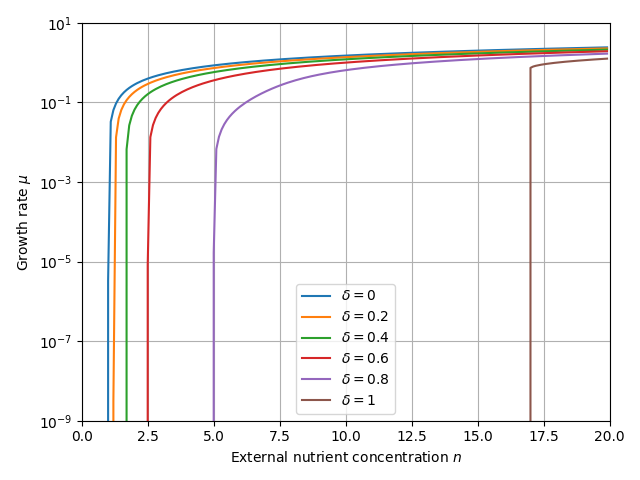
\includegraphics[width=10cm]{n_vs_mu_K1s0_errslope_all.png}
  \caption{エラー率が$x$に式\eqref{errx}の形($K=1$,$\delta=0,0.2,0.4,0.6,0.8,1$)で依存するとして計算した,時刻$t=10^5$における外部栄養濃度$n$と成長速度$\mu$の関係($n$の刻み幅を0.1に変更した.それ以外のパラメータは図\ref{fig:n_vs_mu_errconst}と同様である.).この結果を見ると,$\delta=1$以外は,$\epsilon=\delta/K$とみなしたときの図\ref{fig:n_vs_mu_errconst}と変わらないことが分かる.}
  \label{fig:n_vs_mu_K1s0}
\end{figure}

\begin{figure}[htbp]
  \centering
  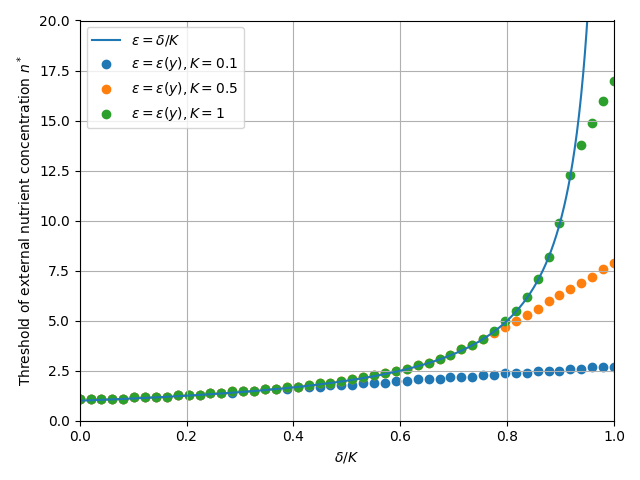
\includegraphics[width=10cm]{err_vs_n_errslope_s0_K.png}
  \caption{エラー率が$x$に式\eqref{errx}の形($K=0.1,0.5,1$)で依存するとして計算した,$\delta$と成長に必要な($\mu > 10^{-3}$となる最小の)外部栄養濃度$n^*$の関係($n$は刻み幅0.1で変更した.それ以外のパラメータは図\ref{fig:n_vs_mu_errconst}と同様である.).これを$\epsilon=\delta/K$のときの理論線と比較すると,$\delta/K$が大きくなるにつれて差が広がることが分かる.また,プロットが理論線から外れ始める$\delta/K$の値は,$K$とともに増加する.}
  \label{fig:err_vs_n_errslope_s0}
\end{figure}